\chapter{Methodology}
\label{chap:2}
\ChapterPageStuff{2}

\section{Preamble}\label{sec:ch2_preamble}
 The literature in \Cref{chap:1} informed the method to create a logging mechanism that captures user-based activity logs to improve software maintenance by analysing the logs obtained. The development of the solution to the identified problem in \Cref{sec:ch1_problemStatement} will be made specifically for a Web-based application.\par Web-based applications are one of the most widely used software implementations that benefit from an analysis of system usage using user-based event logs. These software systems have many different designs. For this study, web applications that require the user to be logged in to an active session in the software system will be used, as seen in \Cref{fig:ch2_webSystemBasic}.

 \begin{figure}[!htb]
	\centering % cent the figure
	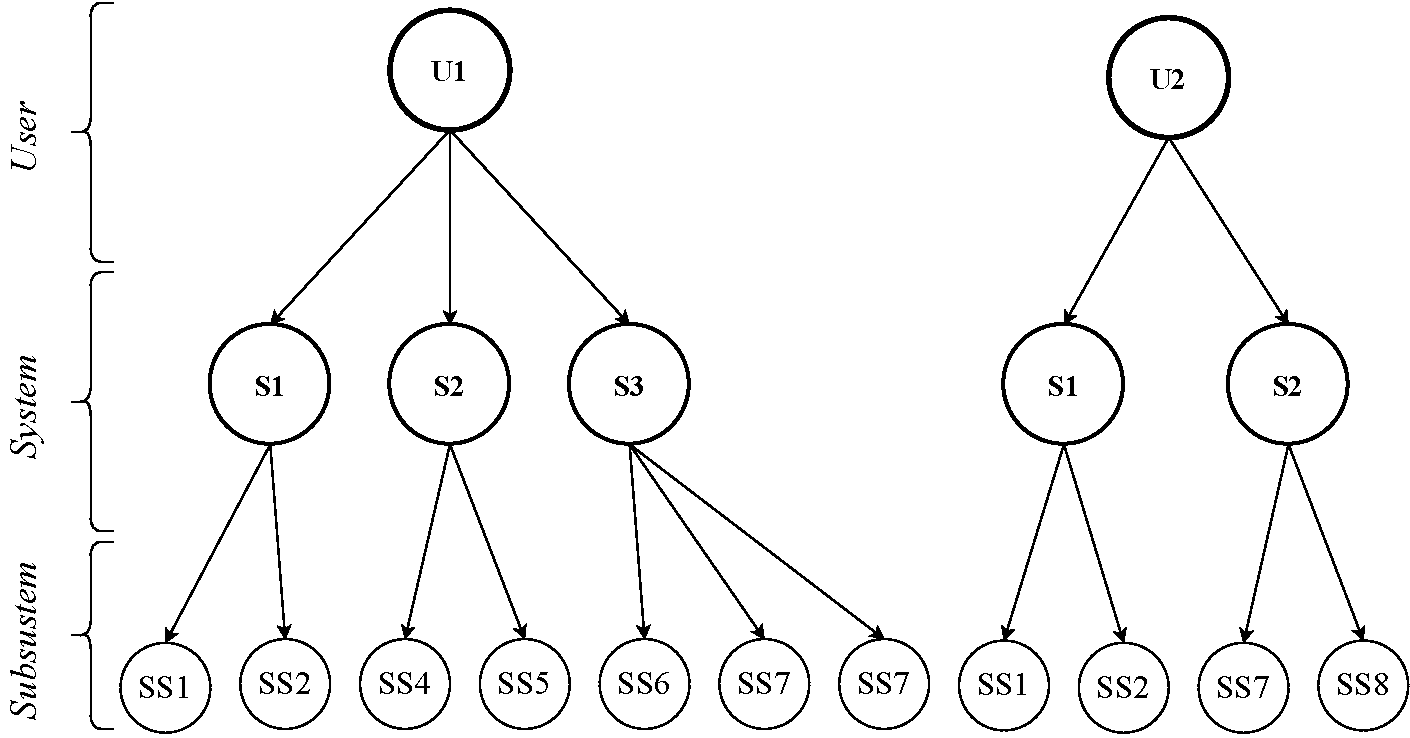
\includegraphics[width=0.95\textwidth]{img/Chapter2/systemOverview/systemOverview.pdf}
	\caption[Basic design of a software system]
	{\textit{Basic design of a software system}}\label{fig:ch2_webSystemBasic}
\end{figure}
 
\Cref{fig:ch2_webSystemBasic} is the basic design of the web application users interact with in different systems. Examples of these systems include the various pages or sections of the website and can be further divided into subsystems. \Cref{sec:ch2_investigate} discusses the method to create a logging mechanism to capture user-generated events is discussed for web-based applications. The different functional requirements and interfaces are also discussed in this section \cite{Anish2015}. \par \Cref{sec:ch2_logAnalysisTools,sec:ch2_utilisationImprovements} discuss the method used to analyse the obtained logs to improve software maintenance using various visualisation tools or available log attributes. \Cref{fig:ch2_systemDesign} illustrates the design for the logging mechanism to capture the user-based event logs.

 \clearpage

 \begin{figure}[!htb]
	 \centering % cent the figure
	 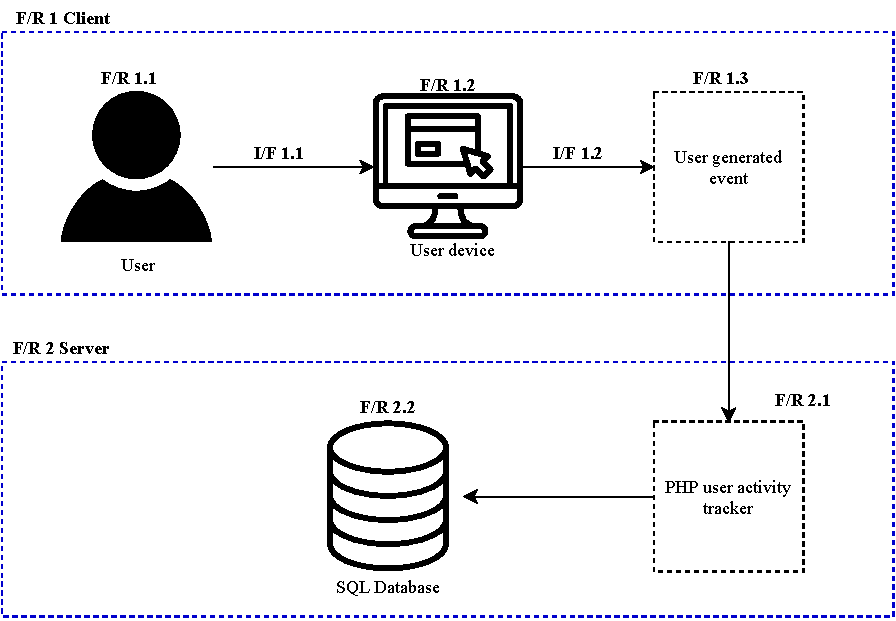
\includegraphics[width=0.95\textwidth]{Chapter2/SystemA_Architecture_Diagram/SystemA_Architecture_Diagram.pdf}
	 \caption[Logging mechanism basic system design]
	 {\textit{Logging mechanism basic system design}}\label{fig:ch2_systemDesign}
 \end{figure}
 
\Cref{fig:ch2_systemDesign} illustrates the basic system design of the logging mechanism. This design provides a high-level overview of the interaction the user has with the software system to create a user-based event log. The two sides of the design in \Cref{fig:ch2_systemDesign} compromise:
 
 \begin{itemize}
	 \item The client side, which involves the user, the device the user uses to access the website and the user-generated event. The user interacts with the website and this creates a user event that can be captured. 
	 \item The server side which has the rest of the user activity logging software that consists of or a single or multiple logging points. The user activity logger interacts with a structured database to store the captured log created from the captured log attributes.
 \end{itemize}

 \clearpage

\section{Development of the solution}\label{sec:ch2_developementOfSolution}
For this study, the development of the solution comprises four main phases:

\begin{itemize}
	\item \textit{Investigate} use methods in the literature or create new methods for a logging mechanism and log-maintenance prioritisation analysis,
	\item \textit{design} a logging mechanism that to performs software prioritisation log analysis,
	\item \textit{verify} whether the solution meet the design specifications, and
	\item \textit{implement} the solution in case studies to evaluate the results.
\end{itemize}

\Cref{fig:ch2_developmentOfSolution} illustrates how these four development parts of the solution are used to create the methodology for this study.

\begin{figure}[!htb]
	\centering % cent the figure
	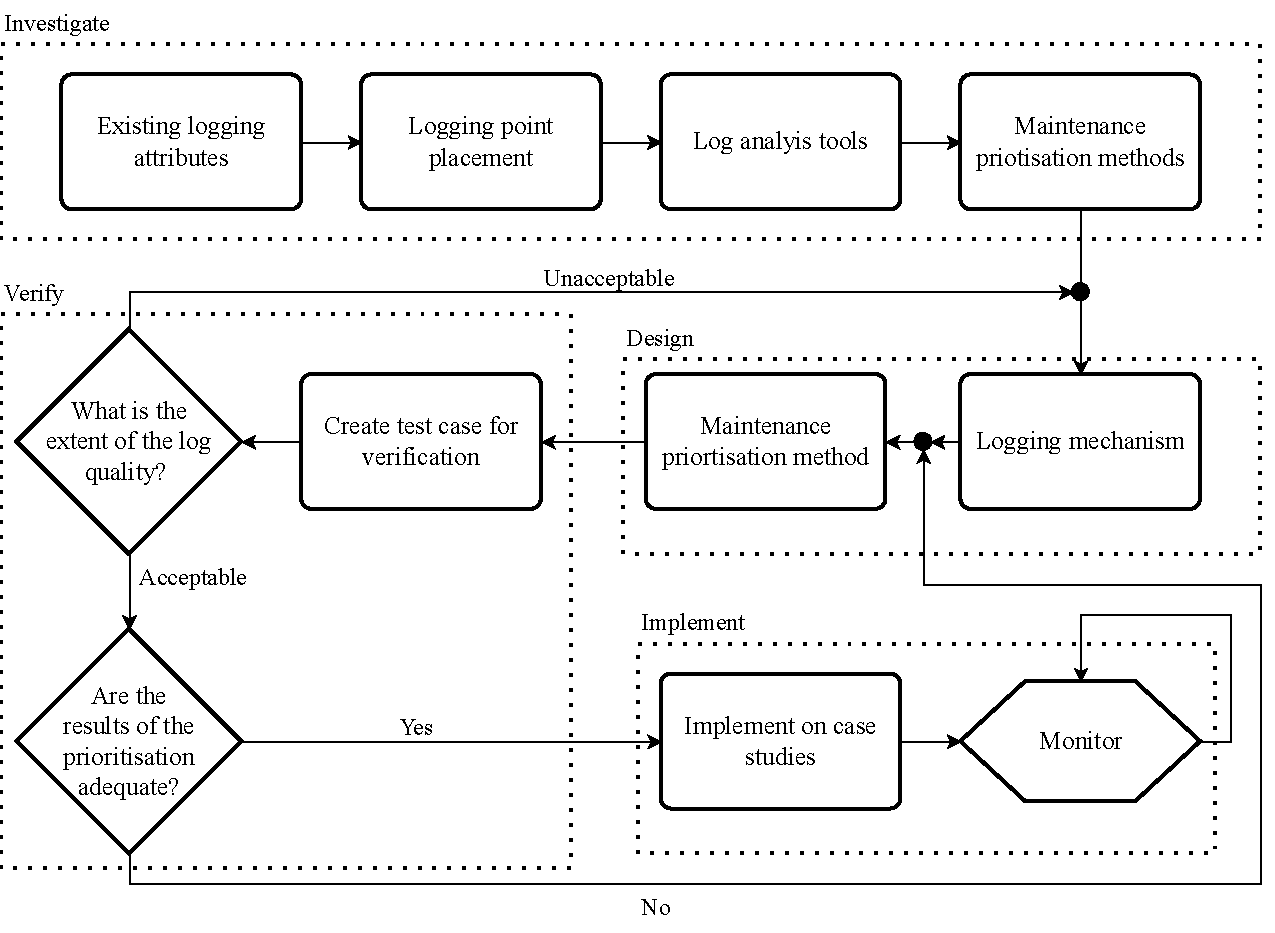
\includegraphics[width=0.95\textwidth]{img/Chapter2/developmentOfSolution/developementOfSolution.pdf}
	\caption[Development of solution]
	{\textit{Development of solution}}\label{fig:ch2_developmentOfSolution}
\end{figure}

The first phase in \Cref{fig:ch2_developmentOfSolution} is the investigation in \Cref{sec:ch2_investigate} to define the requirements for the logging mechanism and the prioritisation of software maintenance using the literature outlined in \Cref{sec:ch1_stateOfArtSection}. \Cref{sec:ch2_design} discusses the second phase, the designing of the logging mechanism as well as the priortising of the software maintenance. 

\clearpage

The verification phase focuses on implementing the design specifications of the logarithmic machinery method and the software maintenance method. The implementation phase follows the verification phase whereby the methods are implemented on the case studies to obtain results that are further monitored and discussed.

\section{Investigate}\label{sec:ch2_investigate}
In this section, functional requirements will be created for the logging mechanism and prioritisation of software maintenance. \Cref{tbl:ch2_developmenetRequirements} is the summary of each of the main functional development requirements created from the investigation phase in \Cref{fig:ch2_developmentOfSolution}. \par The functional requirements (\textbf{F/R}) in \Cref{tbl:ch2_developmenetRequirements} are used to identify each requirement for the development of a solution that can later be verified. Sub-requirements will use the same labelling. 

\setcounter{phase}{0}
\begin{xltabular}{\textwidth}{llX}
	\caption[Functional requirements of the solution]{\textit{Functional requirements of the solution}}\label{tbl:ch2_developmenetRequirements} \\ 
	\toprule
	\thead{Req. ID} & \thead{Name} & \thead{Description} \\
	\midrule
	\endfirsthead

	\caption[]{\continueCaption} \\
	\toprule
	\thead{Req. ID} & \thead{Name} & \thead{Description} \\
	\midrule
	\endhead

	\midrule
	\multicolumn{3}{r}{\continueText} \\ 
	\endfoot
	\endlastfoot

	\rowcolor{lightgray}
	\phase{fr:logAttributes} & Identify log attributes & \RaggedRight The logarithmic attributes must be identified as necessary to complete the log analysis for the prioritisation of software maintenance. The log attributes form the characteristics of the obtained event, herein referred to as on user-based events. \\

	\phase{fr:loggingPoints} & Logging point creation & \RaggedRight Logging points capture the desired log attributes when a user-based event takes place. In \Cref{sec:ch1_loggignPoints} logging points should be strategically placed in the software system to capture the event logs. This stage of development includes identifying where log points should be placed, creating logs, and interacting with the database. \\

	\rowcolor{lightgray}
	\phase{fr:logAnalysis} & \RaggedRight Log analysis tools & Make use of suitable third-party tools or create software to do log analysis on the stored event logs. \\

	\phase{fr:maintenancePrioritising} & \RaggedRight Maintenance prioritising & Create a maintenance prioritising report based on the log analysis for software maintenance using the log analysis tool. The report aims to visualise the use of certain parts of the system and determine maintenance prioritisation. \\
	\bottomrule
\end{xltabular}

The design of the logging mechanism system will be defined in this section to create a generic method for creating a suitable logging mechanism to capture specific user-based event logs. Additionally, this defines any other subfunctional requirements to identify log attributes (\ref{fr:logAttributes}) and the creation of log points (\ref{fr:loggingPoints}).

\subsection{Log attribute requirements}\label{sec:ch2_logAttributesRequirements}
The functional requirement of log attributes (\ref{fr:logAttributes}) focuses on the possible events with which the user has been involved when interacting with the software system. \Cref{tbl:ch2_loggingAttributesFunctionalRequirements} outlines the functional requirements of \ref{fr:logAttributes}.

\setcounter{phase}{1}
\begin{table}[!htb]
	\centering
	\caption[Log attributes functional requirements (\ref{fr:logAttributes})]
	{\textit{Log attributes functional requirements (\ref{fr:logAttributes})}}
	\label{tbl:ch2_loggingAttributesFunctionalRequirements}
	\begin{tabularx}{\textwidth}{lp{3cm}X}
		\toprule
		\thead{Req. ID} & \thead{Name} & \thead{Description} \\
		\midrule

		\rowcolor{lightgray}
		\subphase{fr:userEventReq} & \RaggedRight User-based event log characteristics & \RaggedRight This functional requirement defines the characteristics of what software system events can be classified as a user-based event. \\
  
		\subphase{fr:userActReq} & \RaggedRight User activity types & \RaggedRight User activity types further expand on what event types are valid for \ref{fr:userEventReq}. This is also the first categorisation of the logs obtained. \\ 
  
		\rowcolor{lightgray}
        \subphase{fr:subLogAttributes} & \RaggedRight Log attributes & \RaggedRight The log attributes are the data obtained that describe a log of user-based events. These are the primary data that will be stored in a structured database.\\
		\bottomrule
	\end{tabularx}
\end{table}

\Cref{tbl:ch2_loggingAttributesFunctionalRequirements} is the first functional requirement for the development of a solution that must be defined. It is important to define and create the characteristics of an event log for a user-based event log. 

\subsubsection{User-based event log characteristics}\label{sec:ch2_requirementsOfUAT}
The user is the initiator of the logging mechanism. Each action or event that they trigger by interacting with the user interface on their device can be a potential user-generated event. \Cref{tbl:ch2_requirementsForUserActivtyEvent} outlines the subrequirements for the user that the event log should fulfil to be classified as a user-based activity log.

\setcounter{phase}{1}
\setcounter{subphase}{1}
\begin{xltabular}{\textwidth}{lX}
	\caption[Requirements for an event to be classified as a user-based activity]{\textit{Requirements for an event to be classified as a user-based activity}}\label{tbl:ch2_requirementsForUserActivtyEvent} \\
	\toprule
	\thead{Req. ID} & \thead{Description}\\
	\midrule
	\endfirsthead

	\caption[]{\continueCaption} \\
	\toprule
	\thead{Req. ID} & \thead{Description}\\
	\midrule
	\endhead

	\midrule
	\multicolumn{2}{r}{\continueText} \\ 
	\endfoot
	\endlastfoot

	\rowcolor{lightgray}
	\subsubphase{fr:requirementsUserBased1} & The event must be triggered by the user interacting with the user interface using their device and not any other events that the system self-initiates. The user needs to have interacted directly with the UI. This can also be validated by tracking whether the user did interact with the UI of the HTML element ids. \\

	\subsubphase{fr:requirementsUserBased2} & The event must consist of different cases ($ca~\epsilon~CA$ the cases consist of events) that are noteworthy to make the event log identifiable \cite{Slaninova2014}. \\

	\rowcolor{lightgray}
	\subsubphase{fr:requirementsUserBased3} & For certain types of event logs for \ref{fr:requirementsUserBased2}, the user-generated event should have an origin from which the event took place. \\

	\subsubphase{fr:requirementsUserBased4} & The event log should consist of attributes that expand the identity of the user-based activity. \\

	\rowcolor{lightgray}
	\subsubphase{fr:requirementsUserBased5} & The event must have the user as the initiator or input for the user-based activity. This will exclude all events triggered by the system, as the user did not directly initiate the event. \\
	
	\subsubphase{fr:requirementsUserBased6} & Only use the first \textit{HTTP request}\footnote{A \textbf{HTTP request} is made by a client, to a named host, which is located on a server. The request aims to access a resource on the server.} that is sent to the server. \\ 
	\bottomrule
\end{xltabular}

Every interaction the user has with the user interface of the device to the software system can be seen as an event triggered by the user. Most of these events will not have a meaningful impact as they will not fulfil \ref{fr:requirementsUserBased2} and \ref{fr:requirementsUserBased4} in \Cref{tbl:ch2_requirementsForUserActivtyEvent}.

\clearpage

For the user activity event to meet the requirement of \ref{fr:requirementsUserBased2} it has to have defined cases that describe the activity type of each event. These activity types form the basic criteria for which events can be parsed, which significantly reduces the number of logs that will be obtained. This will ensure that the event logging process will produce quality user-based logs as discussed in \Cref{sec:ch1_loggingQuality}:

\begin{itemize}
	\item A basic structural complexity to simplify log parsing and development of the logging points in the system,
	\item keep the logging consistent by not deviating from the defined cases, and
	\item ensure that the event log's other attributes are complete and available to increase the accuracy and trustworthiness of the event logging when further system utilisation analysis needs to be done. 
\end{itemize}

\subsubsection{User activity types}\label{sec:ch2_userActivityTypes}
The user activity types (\ref{fr:userActReq}) categorise different user-based event logs when they are obtained before other log attributes are fully defined. \Cref{tbl:ch2_userActivityTypes} outlines the functional requirements of the basic user activity types.

\stepcounter{subphase}
\begin{table}[!htb]
	\centering
	\caption[User activity types]
	{\textit{User activity types}}
	\label{tbl:ch2_userActivityTypes}
	\begin{tabularx}{\textwidth}{llX}
		\toprule
		\thead{Req. ID} & \thead{Activity Type} & \thead{Description} \\
		\midrule

		\rowcolor{lightgray}
		\subsubphase{fr:uatType1} & Web page accessed & The user may navigate through different web pages in a session. This tracks when the user first accessed a certain web page or software system on the page. \\


		\subsubphase{fr:uatType2} & Session changes & This is any user activities excluding \ref{fr:uatType1} that modifies the user's session:
		\begin{itemize}
			\item Logging into a web application, both successful and failed attempted log-ins. This user-based activity may cause the log attributes that identify the user and will be a \texttt{NULL} value as the user's session has not started yet,
			\item Ending their session by logging out or declining to extend their session when it is about to expire,
			\item Modifying any session or other relevant variables that can be used in the utilisation analysis
		\end{itemize}\\

		\rowcolor{lightgray}
		\subsubphase{fr:uatType3} & General activity & Any events excluding the first two types of user-based activity that the user initiates when they interact with the web page. Most user activity logs will
		have this event type.\\ 
		\bottomrule
	\end{tabularx}
\end{table}

\clearpage

The general type of user activity event (\ref{fr:uatType3}) will be the most common user activity event and will be catergorised up into different user activity events. \par These user activity types can be further expanded with the general activity (\ref{fr:uatType3}) for log analysis purposes. The general activity types will be different for each system based on what the system enables the user to do or what is needed for further system utilisation analysis, such as determining whether the action the user triggered was to generate a report they downloaded.

\subsubsection{Log attributes}\label{sec:ch2_logAttributes}
The log attributes (\ref{fr:subLogAttributes}) are the descriptive characteristics of the user-based event logs. The functional requirements for the log attributes are defined in \Cref{tbl:ch2_keyLoggingAttributes}.

\stepcounter{subphase}		
\begin{xltabular}{\textwidth}{llX}
    \caption[Logging attributes]{\textit{Logging attributes}}\label{tbl:ch2_keyLoggingAttributes} \\ 
    \toprule
    \thead{Req. ID} & \thead{Logging point} & \thead{Description} \\
    \midrule
    \endfirsthead

    \caption[]{\continueCaption} \\
    \toprule
    \thead{Req. ID} & \thead{Logging point} & \thead{Description} \\
    \midrule
    \endhead

    \midrule
    \multicolumn{3}{r}{\continueText} \\
    \endfoot
    \endlastfoot

    \rowcolor{lightgray}
    \subsubphase{fr:lpa1} & Identification number & The activity identification is an incremental number of the user-based event that is logged. \\
    
    \subsubphase{fr:lpa2} & Timestamp & This is the time the user initiated the user-based activity event. This will be the timestamp from which the log was written in the database, since the log will be made before the rest of the intended \textit{HTTP request} is completed. \\

    \rowcolor{lightgray}
    \subsubphase{fr:lpa3} & Activity type & Each event can be classified into user-based types. This is the type of activity based on users in \Cref{tbl:ch2_userActivityTypes}. \\

    \subsubphase{fr:lpa4} & User identification & Each user has a unique identification number that links the event to them if their session has been verified and can be obtained. It will not be available when the user tries to log in to the system as their session has not yet been set. \\

    \rowcolor{lightgray}
    \subsubphase{fr:lpa5} & Request origin & In web applications, there are always requests sent back to the server which will call the primary function to handle the request. This can be logged as either the file from which the request is sent or the web page from which the request came. \\ 

	\subsubphase{fr:lpa6} & Metadata & The metadata of the event contain request parameters or other relevant request data of the event. These metadata add more information about the user's activity. Some of the event types may not have metadata added. \\

    \rowcolor{lightgray}
    \subsubphase{fr:lpa7} & Miscellaneous & These are any non-metadata attributes that can be consistently captured to for use in the use analysis. They expand the characteristics of the log obtained from the user beyond the base attributes. \\ 
    \bottomrule
\end{xltabular}

The logging attributes defined in \Cref{tbl:ch2_keyLoggingAttributes} are the base attributes that make up the main structure of the user-based event log. For web-based applications on the client side, only some of these attributes can be obtained, as the rest of the attributes can be resolved on the server side. The metadata (\ref{fr:lpa6}) may consist of the request parameters that are available on the server side, but any additional captured data can be added and sent to the server. \par Each of these log attributes combined creates the base log from which key logging points can be created in the software system to capture user-based activity logs in \Cref{tbl:ch2_keyLoggingAttributes}. The activity type (\ref{fr:lpa3}) can be assigned during the user-based activity identification phase with a default value and resolved to a new activity type based on metadata or other parameters by:

\begin{itemize}
	\item Altering any of the session variables that are relevant to the system utilisation analysis,
	\item accessing a certain part of the software system that needs all the user-based activities set to a certain type based on the nature of the procedures that need to be executed such as triggering a generation of a report that can be its user-based activity type, and
	\item sorting teh activity type by HTML element tags, such as a button or text box.
\end{itemize}

\clearpage

Additional parameters may be captured on the client side, such as by the logging point, or they may be captured on the server side when the rest of the log's attributes are being obtained. These extra parameters are shown in \Cref{fig:ch2_MetadataJsonExample}.

\begin{lstlisting}[style=json, caption={\textit{Metadata JSON}}, label={fig:ch2_MetadataJsonExample}] 
	{ "RequestTarget" : "/Area4/Controller4/TestFunction",
		"RequestElementID" : "Button4",
		"RequestParameters": {
			"Parameter1": 4,
			"Parameter2": "Hello World!",
			"Parameter3": true
			"Parameter4": 40.404
			"Parameter5": {
				"Parameter6": "Car",
				"Parameter7" 160000.00
			}
		}		
	}
\end{lstlisting}

The metadata in \Cref{fig:ch2_MetadataJsonExample} is a possible additional parameters that can be obtained for the user-based activity log. The metadata will need to store as a JSON string because it can be a complex object that does not have a set number of parameters. This complex object can have:

\begin{itemize}
	\item The \texttt{RequestTarget} parameter which can be a file path for the website code from which the page is created or a software system. It also contains the function that is called by the \textit{HTTP request}.
	\item The \texttt{RequestElementID} which is the HTML element ID with which the user interacted that caused the user-based activity. This can be used as additional validation that the event was caused by the user. Some of the user-based activities can be certain of these HTML element types by getting the HTML element tag.
	\item The \texttt{RequestParameters} which are all the parameters in the \textit{HTTP request} that can be serialised into a JSON string. This can be used to determine what the user tried to do using this input for the specific function that is used for \ref{fr:requirementsUserBased6} in \Cref{tbl:ch2_requirementsForUserActivtyEvent}.
\end{itemize}

\clearpage

\subsection{Logging point requirements}\label{sec:ch2_serverFunctionalRequirements}
The functional requirement of the logarithmic point (\ref{fr:loggingPoints}) focuses on the creation and strategic placement of the logarithmic points. The log points that obtain the log attributes must also store the created event log in a structured database. The logging point's subfunctional requirements are defined in \Cref{tbl:ch2_loggingPointsFuntionalRequirements}. 

\stepcounter{phase}
\begin{table}[!htb]
	\centering
	\caption[Logging points functional requirements (\ref{fr:loggingPoints})]
	{\textit{Server functional requirements (\ref{fr:loggingPoints})}}
	\label{tbl:ch2_loggingPointsFuntionalRequirements}
	\begin{tabularx}{\textwidth}{llX}
		\toprule
            \thead{Req. ID} & \thead{Name} & \thead{Description} \\
            \midrule

            \rowcolor{lightgray}
		\subphase{fr:serverActivityLogger} & Logging point placement & The logging points are used to capture and create the user-based event log that will be stored in a database.\\
  
		\subphase{fr:serverDatabase} & Storing the user-based activity logs & The event log is stored in a structured database until it is needed for further log analysis.\\
		\bottomrule
	\end{tabularx}
\end{table}

\Cref{tbl:ch2_loggingAttributesFunctionalRequirements} concludes the design requirements for the logging mechanism. The stored logs will be further processed when the log analysis needs to be implemented.

\subsubsection{Logging point placement}\label{sec:ch2_loggingPoints}
Additional to \Cref{sec:ch1_loggignPoints}, the logging points should be strategically placed in the software system to capture the log attributes for the user-based activity log. To meet the requirements of \Cref{tbl:ch2_requirementsForUserActivtyEvent} for a user-based activity, the log points should adhere to the functional requirements of the log points of \Cref{tbl:ch2_loggingPointRequirement}.

\setcounter{phase}{2}
\setcounter{subphase}{1}
\begin{table}[!htb]
	\centering
	\caption[Logging point requirements]
	{\textit{Logging point requirements}}
	\label{tbl:ch2_loggingPointRequirement}
	\begin{tabularx}{\textwidth}{lX}
		\toprule
		\thead{Req. ID} & \thead{Description} \\
		\midrule

            \rowcolor{lightgray}
		\subsubphase{fr:lp1} & The logging point should be placed where the user's interaction with the software system will send a \textit{request} back to the server. \\
  
		\subsubphase{fr:lp2} & Each logging point should consistently capture the user-based activity as the activity is happening. \\

            \rowcolor{lightgray}
		\subsubphase{fr:lp3} & Logging points should be globally complete to capture the user-based activities in the given software system without too much modification between each point in the same software system. \\
  
		\subsubphase{fr:lp4} & The logging points should not interfere with the rest of the system's operations; this would slow down the system by causing too much overhead in each \textit{request}
		that is being sent. \\
		\bottomrule
	\end{tabularx}
\end{table}

\clearpage

The logging points can be either a single code segment or consist of multiple code segments in a software system that aim to capture user-based actions as they happen. Creating multiple logging points in a software environment will:

\begin{itemize}
	\item Increase the complexity of the logarithmic mechanism. Each point can be different from the other as it will need certain operations to capture the log,
	\item the consistency of the logging might differ and increase as the logging points increase in a software system, and 
	\item the correctness of the logging will be impacted if the different changes in the logging point are unable to consistently capture the user-based activity or extract all the needed attributes to complete the user-based log.
\end{itemize}

Creating a single logging point reduces the complexity and, in most cases, will improve the consistency and correctness of the user-based logs. In web applications, a globally defined logging point can be used in a modified \textit{HTTP request} that will form the base template for all or most \textit{HTTP request} used in the software system, as discussed in \Cref{sec:ch2_webApplicationArchitecture}. \par The use of a single centralised logging point does not guarantee that the logging mechanism will perform more efficiently and accurately than using multiple logging mechanisms. Using a single logging point may have complexity issues when the logging point needs to capture each user-based activity consistently with different cases.

\subsubsection{Storing the user-based activity logs}\label{sec:ch2_databaseStorage}
After the logging point has captured the log attributes and created the event log, the log can be saved in a structured database. The storing of the functional requirements of user-based logs (\ref{fr:serverDatabase}) should be defined for structured database interactions.\par The captured parameters of the log attributes may have some sensitive user data that should not be logged. Functions can be excluded or assigned a new user activity type that will need to filter out certain parameters or not log any parameters at all, such as:

\begin{itemize}
	\item Session handling functions that contain passwords or other user information that should not be available to anyone but the user. This could lead to unintentional information disclosure of any personal information in the system utilisation analysis if it is available for anyone who can access and use the user-based activity logs, and
	\item complex parameters such as file upload streams of files that the user tries to upload. This information cannot be broken down to a simple \texttt{JSON} structure seen in \Cref{fig:ch2_MetadataJsonExample}. Other metadata such as the file size, name, and type can rather be logged. Detecting these complex parameters allows these types of user-based activities to be defined separately.
\end{itemize}

\Cref{tbl:ch2_SQLLoggingTable} outlines the type of data for the parameters and the functional requirements that it will need to fulfil \Cref{tbl:ch2_keyLoggingAttributes}.

\stepcounter{subphase}
\begin{table}[!htb]
	\centering
	\caption[Log attributes for database storing of the event logs]
	{\textit{Log attributes for database storing of the event logs}}
	\label{tbl:ch2_SQLLoggingTable}
	\begin{tabularx}{\textwidth}{lXX}
            \toprule
		\thead{Req. ID} & \thead{Column Name} & \RaggedRight \thead{Log attribute requirement} \\
            \midrule

            \rowcolor{lightgray}
		\subsubphase{fr:lpd1} & ActivityID & \ref{fr:lpa1} \\
		\subsubphase{fr:lpd2} & Timestamp & \ref{fr:lpa2} \\
            \rowcolor{lightgray}
		\subsubphase{fr:lpd3} & ActivityType & \ref{fr:lpa3} \\
		\subsubphase{fr:lpd4} & UserID & \ref{fr:lpa4} \\
            \rowcolor{lightgray}
		\subsubphase{fr:lpd5} & Subsystem & \ref{fr:lpa5} \\
		\subsubphase{fr:lpd6} & GroupID & \ref{fr:lpa7} \\
            \rowcolor{lightgray}
		\subsubphase{fr:lpd7} & MetaData & \ref{fr:lpa6} \\
		\bottomrule
	\end{tabularx}
\end{table}

In \Cref{tbl:ch2_SQLLoggingTable} the functional requirements of log attributes should match the functional requirements (\ref{fr:serverDatabase}) of the logging attribute (\ref{fr:subLogAttributes}). Any other parameters can be added using the miscellaneous (\ref{fr:lpa7}). \par New tables or other structured storage entities can be added to save the captured data from the logging point. 

\subsection{Log analysis tool}\label{sec:ch2_logAnalysisTools}
The log analysis (\ref{fr:logAnalysis}) uses third-party analytical tools or custom-created software log analysis implementations. Developers should use the implementation that fulfils their log-analysis requirements. \Cref{tbl:ch2_logAnalysis} is the log analysis functional requirements (\ref{fr:logAnalysis}).

\setcounter{phase}{3}
\setcounter{subphase}{0}
\begin{table}[!htb]
	\centering
	\caption[Log analysis functional requirements (\ref{fr:logAnalysis})]
	{\textit{Log analysis functional requirements (\ref{fr:logAnalysis})}}
	\label{tbl:ch2_logAnalysis}
	\begin{tabularx}{\textwidth}{llX}
		\toprule
		\thead{Req. ID} & \thead{Name} & \thead{Description} \\
		\midrule

		\rowcolor{lightgray}
		\subphase{fr:logQuality} & Log quality & \RaggedRight Log quality ensures that the logs obtained are usable for log analysis. Any incomplete logs should be either fixed in the log analysis implementation or the logging mechanism should be adjusted to capture the complete logs. \\
		\subphase{fr:logAnalysisTool} & Log analysis tool requirement & \RaggedRight Certain basic requirements are needed for the log analysis tool to implement a log analysis. \\
		\bottomrule
	\end{tabularx}
\end{table}

\subsubsection{Log quality}
The log quality identified in \Cref{sec:ch1_loggingQuality} is significant when implementing a log-analysis mechanism. Log quality (\ref{fr:logQuality}) will affect both the performance of the logging mechanism and the accuracy and completeness of the log quality. \Cref{tbl:ch2_utilisation_requirements} outlines the functional requirements for log quality (\ref{fr:logQuality}).

\setcounter{phase}{3}
\setcounter{subphase}{1}
\begin{table}[!htb]
	\centering
	\caption[Log quality functional requirements (\ref{fr:logQuality})]
	{\textit{Log quality functional requirements (\ref{fr:logQuality})}}
	\label{tbl:ch2_utilisation_requirements}
	\begin{tabularx}{\textwidth}{llX}
            \toprule
		\thead{Req. ID} & \thead{Requirement name} & \thead{Description} \\
            \midrule

            \rowcolor{lightgray}
		\subsubphase{fr:ur1} & Log availability & \RaggedRight The log attributes should be available when the logging mechanism is actively capturing the user-based events. It should be \textit{locally-} and \textit{globally complete}.  \\
  
		\subsubphase{fr:ur2} & Log completeness & \RaggedRight User-based logs should be complete and minimal corrections should be made after logging during the log extraction process (\ref{fr:ur3}) and presentation of visualisation. \\

            \rowcolor{lightgray}
            \subsubphase{fr:ur3} & Log extraction & \RaggedRight User-based logs are extracted from the database and imported into a visualisation presentation for user-based activity logs. \\
		\bottomrule
	\end{tabularx}
\end{table}

All functional requirements of the user-based activity log in \Cref{sec:ch2_requirementsOfUAT} are achieved with minimal subsequent processing of the raw logs. Changes to the system that impact which possible user-based events are considered for logging are inevitable. \par Log extraction refers to the methods used to obtain the logs from the database with any other relevant data that can be used in the visualisation presentation (\ref{fr:ur4}). The raw logs make use of foreign references to other tables in the database to provide more details on the user-based event log, as seen in \Cref{fig:ch2_erdOfEventLogs}.

\clearpage

\subsubsection{Log analysis tool requirement}
The log analysis tool (\ref{fr:logAnalysisTool}) ensures that a custom or third-party implementation is performed and able to meet some basic log-analysis requirements defined in \Cref{tbl:ch2_logAnalysisToolFR}.

\stepcounter{subphase}
\begin{table}[!htb]
	\centering
	\small
	\caption[Log analysis tool functional requirements (\ref{fr:logAnalysisTool})]
	{\textit{Log analysis tool functional requirements (\ref{fr:logAnalysisTool})}}
	\label{tbl:ch2_logAnalysisToolFR}
	\begin{tabularx}{\textwidth}{llX}
		\toprule
		\thead{Req. ID} & \thead{Requirement name} & \thead{Description} \\
		\midrule

		\rowcolor{lightgray}
		\subsubphase{fr:ur4} & Log visual presentation & The visual presentation of the extracted logs should be shown to the user who will make use of the activity logs in a custom visual system or make use of other third-party tools. This will affect how the logs will be extracted (\ref{fr:ur4}) from the database because third-party systems may use an API to get the logs from the database. \\
  
		\subsubphase{fr:ur5} & Log comparison & \RaggedRight Using \ref{fr:logAnalysisTool}, use different log attributes that are used as defined criteria. This allows different types of users, subsystems, and activity types to be grouped and compared.\\

        \rowcolor{lightgray}
        \subsubphase{fr:ur6} & \RaggedRight Maintenance suggestions & Maintenance suggestions can be made from system utilisation reports by prioritising maintenance or decommissioning software systems. This can be data or visual representations of the logarithmic comparison (\ref{fr:ur5}) using the log visual presentation systems (\ref{fr:ur6}) or creating a summary report from the visual presentation that contains maintenance suggestions. \\
		\bottomrule
	\end{tabularx}
\end{table}

Each of these functional requirements ensures that the system utilisation analysis will be achieved for the created logging mechanism in \Cref{sec:ch2_investigate}. The main user interface of the system usage analysis will consist of the presentation of user-based activities (\ref{fr:ur4}). This system will be either a custom-created system to display these logs or third-party software such as Microsoft's business intelligence platform, PowerBI. \par Using third-party tools has advantages over creating custom software for visual presentation (\ref{fr:ur4}). These include:

\begin{itemize}
	\item \RaggedRight Third-party BI platforms provide all the necessary analytical functionality, making it easy to create visual representations with minimal programming,
	\item \RaggedRight the advanced tools on these platforms offer various approaches to visualise user-based activity logs for log comparison (\ref{fr:ur5}), and
	\item \RaggedRight maintenance and editing of these representations is usually trouble-free, with ample support and guides available for developers to make updates to custom visual presentations.
\end{itemize}

\clearpage

There are, however, disadvantages to using third-party tools. These include:

\begin{itemize}
	\item \RaggedRight Third-party BI platforms are likely to require a subscription, which can be costly for a company licence,
	\item \RaggedRight additional courses may be necessary to fully utilise the capabilities of these platforms, and
	\item \RaggedRight additional functionality may be required for log extraction (\ref{fr:ur3}) to import data into the platform.
	\end{itemize}

With the drawbacks listed above, third-party business intelligence platforms are the better visual presentation tools for the system utilisation analysis if the tools are available for use.

\subsection{Maintenance prioritisation}\label{sec:ch2_utilisationImprovements}
Maintenance prioritisation is performed from logarithmic analysis. Maintenance priority functional requirements (\ref{fr:maintenancePrioritising}) are shown in \Cref{tbl:ch2_maintenancePriortising}.

\setcounter{phase}{4}
\setcounter{subphase}{0}
\begin{table}[!htb]
    \centering
    \caption[Maintenance prioritising functional requirements (\ref{fr:maintenancePrioritising})]
    {\textit{Maintenance prioritising functional requirements (\ref{fr:maintenancePrioritising})}}
    \label{tbl:ch2_maintenancePriortising}
    \begin{tabularx}{\textwidth}{lp{4cm}X}
        \toprule
        \thead{Req. ID} & \thead{Name} & \thead{Description} \\
        \midrule
    
        \rowcolor{lightgray}
        \subphase{fr:systemUtiReq} & \RaggedRight System utilisation analysis categories & \RaggedRight The system utilisation analysis categories are needed to complete logging analysis. These categories will provide the data necessary to make recommendations on how to prioritise software maintenance using these log analysis metrics.\\
  
        \subphase{fr:maintenanceFactor} & \RaggedRight Maintenance prioritisation factor & \RaggedRight The maintenance factor measures the amount of maintenance required for a given software system. This is used to prioritise the software maintenance efforts of the software developers using a scoring system. \\
        
        \bottomrule
    \end{tabularx}
\end{table}

\clearpage

\subsubsection{System utilisation analysis categories}
The system utilisation analysis categories functional requirements (\ref{fr:systemUtiReq}) are used to categorise the log data for maintenance prioritisation metrics. \Cref{tbl:ch2_utilisationCategories} outlines the functional requirements of the system utilisation analysis categories (\ref{fr:systemUtiReq}).

\setcounter{subphase}{1}
\begin{table}[!htb]
    \centering
    \caption[System utilisation analysis categories functional requirements (\ref{fr:systemUtiReq})]
    {\textit{System utilisation analysis categories functional requirements (\ref{fr:systemUtiReq})}}
    \label{tbl:ch2_utilisationCategories}
    \begin{tabularx}{\textwidth}{lp{3cm}X}
        \toprule
        \thead{Req. ID} & \thead{Requirement name} & \thead{Description} \\
        \midrule
    
        \rowcolor{lightgray}
		\subsubphase{fr:utCategories1} & Users & \RaggedRight Users of software systems can be placed in different categories according to who uses the software. This can be both the customer users and the employees using the software. Using the activities of the customer users will provide the data for the development team to need their resources. \\
  
		\subsubphase{fr:utCategories2} & \RaggedRight User activity types & User activity types in \Cref{tbl:ch2_userActivityTypes} can be used as a category to compare different types of user-based activities and use a subcategory for categories such as different users who can use the system (\ref{fr:utCategories1}). \\

        \rowcolor{lightgray}
        \subsubphase{fr:utCategories3} & \RaggedRight Systems or subsystems & \RaggedRight The request origin (\ref{fr:lpa5}) of user-based activities can be classified to compare different subsystems and controllers. \\
    
        \subsubphase{fr:utCategories4} & \RaggedRight Miscellaneous categories & \RaggedRight This user-based activity category will use the metadata attribute (\ref{fr:lpa7}) of \Cref{tbl:ch2_keyLoggingAttributes}. The other fields that are not set as main categories can also be placed in this category because they can take multiple forms.\\
        \bottomrule
    \end{tabularx}
\end{table}

The categories in \Cref{tbl:ch2_utilisationCategories} allow the log data to be placed in different categories for comparison. A software maintenance prioritising model can be made using the comparisons of these categories.

\clearpage

\subsubsection{Maintenance prioritisation factor}
The maintenance prioritisation factor (\ref{fr:maintenanceFactor}) makes use of various parameters created from the logs obtained. This prioritisation factor will need to indicate, for any given subsystem's software maintenance priorisation, using a consistent method to determine the maintenance prioritisation factor. \Cref{tbl:ch2_maintenancePriorFactor} outlines the functional requirement for the maintenance prioritisation factor (\ref{fr:maintenanceFactor}).

\stepcounter{subphase}
\begin{table}[!htb]
    \centering
    \caption[Maintenance priorisation factor functional requirements (\ref{fr:maintenanceFactor})]
    {\textit{Maintenance priorisation factor functional requirements (\ref{fr:maintenanceFactor})}}
    \label{tbl:ch2_maintenancePriorFactor}
    \begin{tabularx}{\textwidth}{lp{3cm}X}
        \toprule
        \thead{Req. ID} & \thead{Requirement name} & \thead{Description} \\
        \midrule
    
        \rowcolor{lightgray}
        \subsubphase{fr:mpr1} & Users & \RaggedRight The total number of users that are active in the subsystems should be a parameter. \\
    
        \subsubphase{fr:mpr2} & Priority & \RaggedRight Priority is a precalculated parameter that indicates the importance of a subsystem. This can be calculated or defined for each subsystem. \\
    
        \rowcolor{lightgray}
        \subsubphase{fr:mpr3} & Activities & \RaggedRight The total number of user activities for a subsystem must be used as an input parameter for the software maintenance factor. \\
    
        \subsubphase{fr:mpr4} & \RaggedRight Software maintenance factor & \RaggedRight The software maintenance factor is the measurement of the importance of a certain software system. This is calculated using \ref{fr:mpr1}, \ref{fr:mpr2}, and \ref{fr:mpr3}. \\
    
        \bottomrule
    \end{tabularx}
\end{table}

A method can be used to determine the prioritisation of software maintenance of each subsystem in a given system using the functional requirements in \Cref{tbl:ch2_maintenancePriorFactor}. The defined parameters provide a basic guideline on the input and output parameters the method needs for the calculations.

\clearpage

\section{Design}\label{sec:ch2_design}
The design of the log mechanism and log analysis will be defined in this section as well as the flow diagrams of the logging mechanism and log analysis.

\subsection{Web application architecture}\label{sec:ch2_webApplicationArchitecture}
To determine the types of user activity for a web application, the architecture of the Web application will be a factor in the logging mechanism. Web applications consist mostly of HTML, JavaScript, and CSS programming languages. The Model-View-Controller (MVC) architecture is mostly used for web-based applications using that programming language \cite{Jailia2016}. The MVC architecture in \Cref{fig:ch2_flowMVC_Architecture} comprises of three basic parts \cite{Jailia2016}:

\begin{itemize}
	\item \textit{Model:} The representation of the records in the database which also interacts with the database through a database access layer or service manipulating the data using the CRUD operations:
	\begin{itemize}
		\item \textit{create} operation that adds new data,
		\item \textit{read} operation that gets the data from the database,
		\item \textit{update} operation that modifies the existing data, and
		\item \textit{delete} operation that removes data.
	\end{itemize}
	\item \textit{Controller:} Operates both the \textit{View} and \textit{Model} and serves as the connection between the user and the system by controlling the data flow of the \textit{View}  and \textit{Model}.
	\textit{View}.
	\item \textit{View:} Indicates the results of the data contained in the \textit{Model} and enables the user to manipulate the data. The user will only interact with this part of the web application.
\end{itemize}

\begin{figure}[!htb]
	\centering % cent the figure
	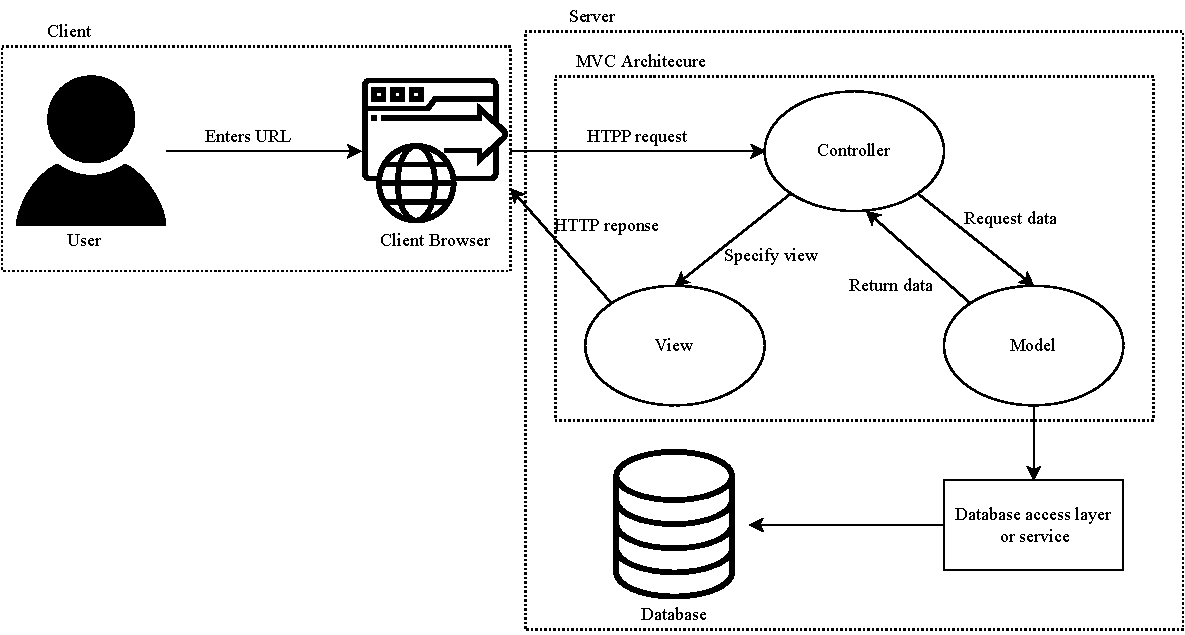
\includegraphics[width=0.96\textwidth]{Chapter2/Flow_MVC_Architecture/Flow_MVC_Architecture.pdf}
	\caption[MVC architecture for most web-based applications]
	{\textit{MVC architecture for most web-based applications \cite{Gu2010}}}\label{fig:ch2_flowMVC_Architecture}
\end{figure}

\Cref{fig:ch2_flowMVC_Architecture} illustrates the equivalent representation of the MVC architecture of \Cref{fig:ch2_systemDesign} where the data flow of the MVC architecture is shown. The user interacts with the web application through their browser which sends a \textit{HTTP requests} to the \textit{Controller} and receive a \textit{HTTP response}\footnote{An \textbf{HTTP response} is made by a server to a client. The response aims to provide the client with the resource it requested, inform the client that the action it requested has been carried out, or else inform the client that an error occurred in processing its request. Refer to the source: IBM, "HTTP responses", IBM, Available: \url{https://www.ibm.com/docs/en/cics-ts/5.2?topic=protocol-http-responses} (visited on 2023-07-24)} from the \textit{View}. The \textit{Controller} will request and return the data to the \textit{Model} which interacts with the database access layer or service to do the \textit{create}, \textit{update}, and \textit{delete} operations. \par To classify any interaction between the user (\ref{fr:logAttributes}) and the server (\ref{fr:loggingPoints}) to meet the functional requirements of \Cref{tbl:ch2_requirementsForUserActivtyEvent}, only the \textit{HTTP request} is used for the logging points in \Cref{sec:ch2_loggingPoints} because:

\begin{itemize}
	\item It meets \ref{fr:requirementsUserBased1} and \ref{fr:requirementsUserBased1} when the user interacts with \textit{ View} to modify the data that must be sent as back an \textit{HTTP request} to process the data on the \textit{Controller},
	\item The user activity types can be assigned for different scenarios the user triggers when the request is sent, and 
	\item any additional metadata can be sent with the \textit{request header}\footnote{A \textbf{request header} is an HTTP header that can be used in an HTTP request to provide information about the request context so that the server can tailor the response. For example, the Accept-$\ast$ headers indicate the allowed and preferred formats of the response. Refer to the source: MDN Web Docs, "Request header", MDN Web Docs, Available: \url{https://developer.mozilla.org/en-US/docs/Glossary/Request_header} (visited on 2023-07-24)} of the \textit{HTTP request}. This will reduce the overhead added by the logging mechanism by not sending an additional \textit{HTTP request} back to the server each time a user-based activity has been identified.
\end{itemize}

\clearpage

\subsection{Server-side logging point}\label{sec:ch2_serverSideLoggingpoint}
\Cref{sec:ch2_loggingPoints} discusses the functional requirements for the logging point that must be met to create a suitable logging point for a software system to track user-based activities. The \textit{HTTP request} will call a function in the system, subsystem, or web page to execute the user's actions. This \textit{request} information can then be obtained and parsed onto the logging point. \par The logging attribute can be created as a centralised code segment that all the software system's components can execute before executing the targeted software system in web applications such as. These centralised code systems comprise:

\begin{itemize}
	\item In most software frameworks, the \textit{HTTP request} data can be extracted from the inbuilt \textit{HTTP request} models to obtain the custom request headers set on the client side. There should be at least one common global location in the software where a single log point can be called for every \textit{HTTP} function to execute the log point first before continuing with the rest of the main targeted function. The rest of the log attributes can also be obtained during the execution run time:
	\begin{itemize}
		\item \textbf{Absolute URI path:} The string containing the absolute URI path of the currently active system, subsystem, or web page. 
		\item \textbf{Absolute request URL:} The requested URL contains the target system, subsystem, or web page name and function that the request needs to be executed. 
		\item \textbf{Action parameters:} During the execution time some of the parameters which are the request parameters sent with the \textit{HTTP request} from the client device can be obtained.
	\end{itemize}
	\item In other older web applications that are created with programming languages such as \texttt{PHP} a more direct approach needs to be taken when accessing the request data. In this case, multiple logging points are used that call the logging points' main code segment to capture the attributes and store the log in a database. The parameters may need to be extracted before parsing them into the main logging point code segment.
\end{itemize}

As long as the logging attributes and the \textit{HTTP request} headers are obtainable, the logging mechanism can be created on the server side to extract and process the data. The activity type can be resolved by the defined cases; for example, if the request calls the \texttt{Index} function of the system, subsystem or webpage, it can be identified as the web page accessed user activity type (\ref{fr:uatType1}) of \Cref{tbl:ch2_userActivityTypes}. \par If the user-based event is using the system, subsystem, web page, or functions that modify the session, it can be classified as a session changed event (\ref{fr:uatType3}). Subsequently, the remaining user-based activity events need to be tested if they meet certain criteria defined for the general activity types. If user-based event fails all three types of classification, the event is likely not user-generated or comes from a \textit{HTTP request} that was executed after the initial first request. In such cases, the last HTML element id that triggered the event should not be listed as a clicked element in JavaScript.

\subsection{Client functional requirements interaction}
\Cref{fig:ch2_user_based_actvity_classification} illustrates the complete process of the user interacting with the user interface to trigger a user-based activity event to be logged later for the client's functional requirements. The process starts with the user interacting with the user interface. The default activity type is set to general activity (\ref{fr:uatType3}) until it is further processed later in the logging mechanism. \par If the activity has additional metadata such as other request parameters, it will be logged by adding it to the search for it in the completion of the \textit{HTTP request} operation. The additional metadata can also be captured in this stage from the client side, such as the element that the user clicked to initiate the event. The captured metadata are then placed in a custom request header, and the \textit{HTTP request} continues its normal operations and sends the data back to the server.

\clearpage

\begin{figure}[!htb] % An h :here, t: top, b: bottom.
	\centering % cent the figure
	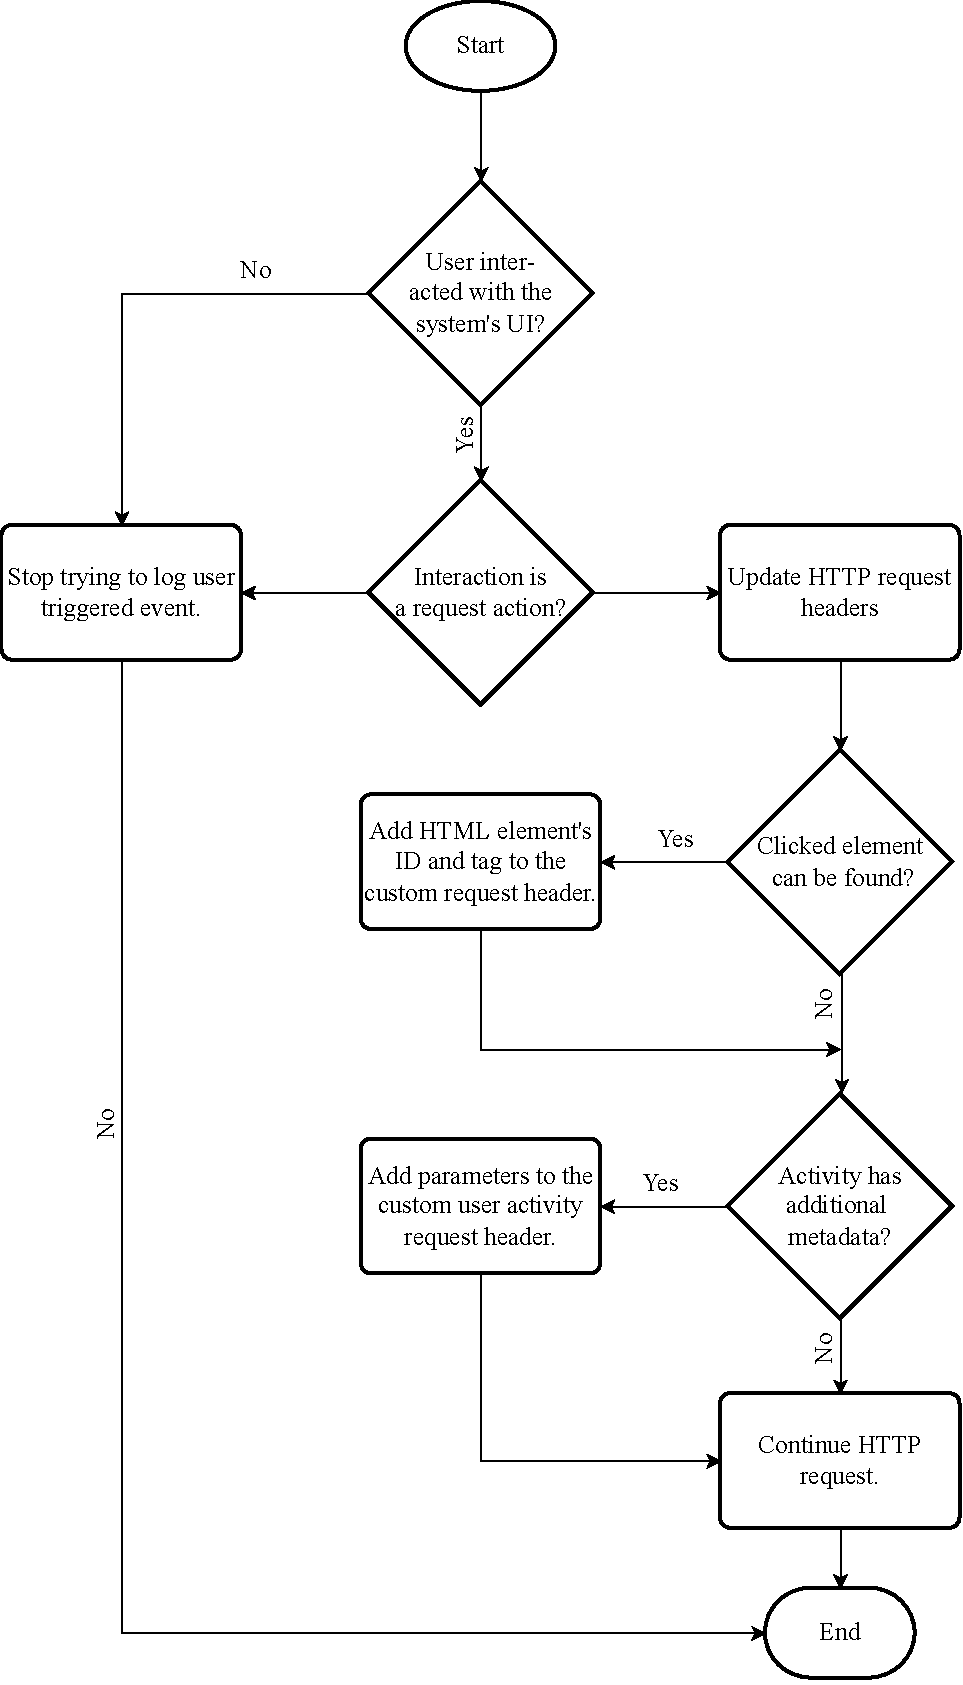
\includegraphics[width=0.75\textwidth]{Chapter2/user_based_flow_diagram/user_based_flow_diagram.pdf}
	\caption[User-based activity log classification flow diagram]
	{\textit{User-based activity log classification flow diagram}}\label{fig:ch2_user_based_actvity_classification}
\end{figure}

\clearpage

\subsection{Server-side log parsing}
\Cref{fig:ch2_loggingParse} illustrates the server-side log parsing of the possible user-based activity events obtained for the software system.\par The defined globally-set logging point will start the user-based activity process before the targeted process \Cref{fig:ch2_loggingParse} is executed. At this stage, if something goes wrong with the logging during the execution of this filter, it should be abandoned and the software system should be left to continue to ensure that it does not interfere with the software system's operations (\ref{fr:lpa4} of \Cref{tbl:ch2_loggingPointRequirement}). \par In the case of the request method \texttt{NULL} or empty due to errors such as incorrect parameter types for the targeted procedure in the controller, the logging point should stop attempting to log the user-based log. The issue would most likely appear as a runtime error and any user-based activity log procedures will likely fail due to incomplete data or render the logs incomplete or inconsistent (\ref{fr:lpa3} of \Cref{tbl:ch2_loggingPointRequirement}). \par If the captured user-activity log contains any parameters, it should be checked for any session-related parameters or any other potential user data that should be removed from the metadata to prevent any personal information from being accessed by anyone who is not the owner of the user account. If the user-activity does not contain any request parameters, \texttt{ElementsInfo} should be set to \texttt{NULL}.\par In \Cref{fig:Ch2_ElementInfo} is the \texttt{JSON} data of \texttt{ElementInfo}. 

\begin{lstlisting}[style=json, caption={\textit{Element properties JSON}}, label={fig:Ch2_ElementInfo}] 
	{ "ElementTagName" : "button",
		"ElementID" : "submitButton",
		"ElementDataKey": "submit-control"		
	}
\end{lstlisting}

Each of the properties in \Cref{fig:Ch2_ElementInfo} consist of:

\begin{itemize}
	\item \texttt{ElementTagName}, is the HTML element's tag name which is one of the defined accepted tag names, such as \texttt{button}, \texttt{label}, and \texttt{td} etc.,
	\item \texttt{ElementID} is the, identification of the element if it has been assigned to the element and can be obtained on the client side, and
	\item \texttt{ElementDataKey} is, additional captured data attributes that expand on the identity of the element if it is a custom-made HTML element control. Some software systems may have other custom-created HTML elements, which can also trigger a user-based activity. There may be other miscellaneous elements, such as a \texttt{label}, which are not normal input controls.
\end{itemize}

\clearpage

\begin{figure}[!htb]
	\centering
	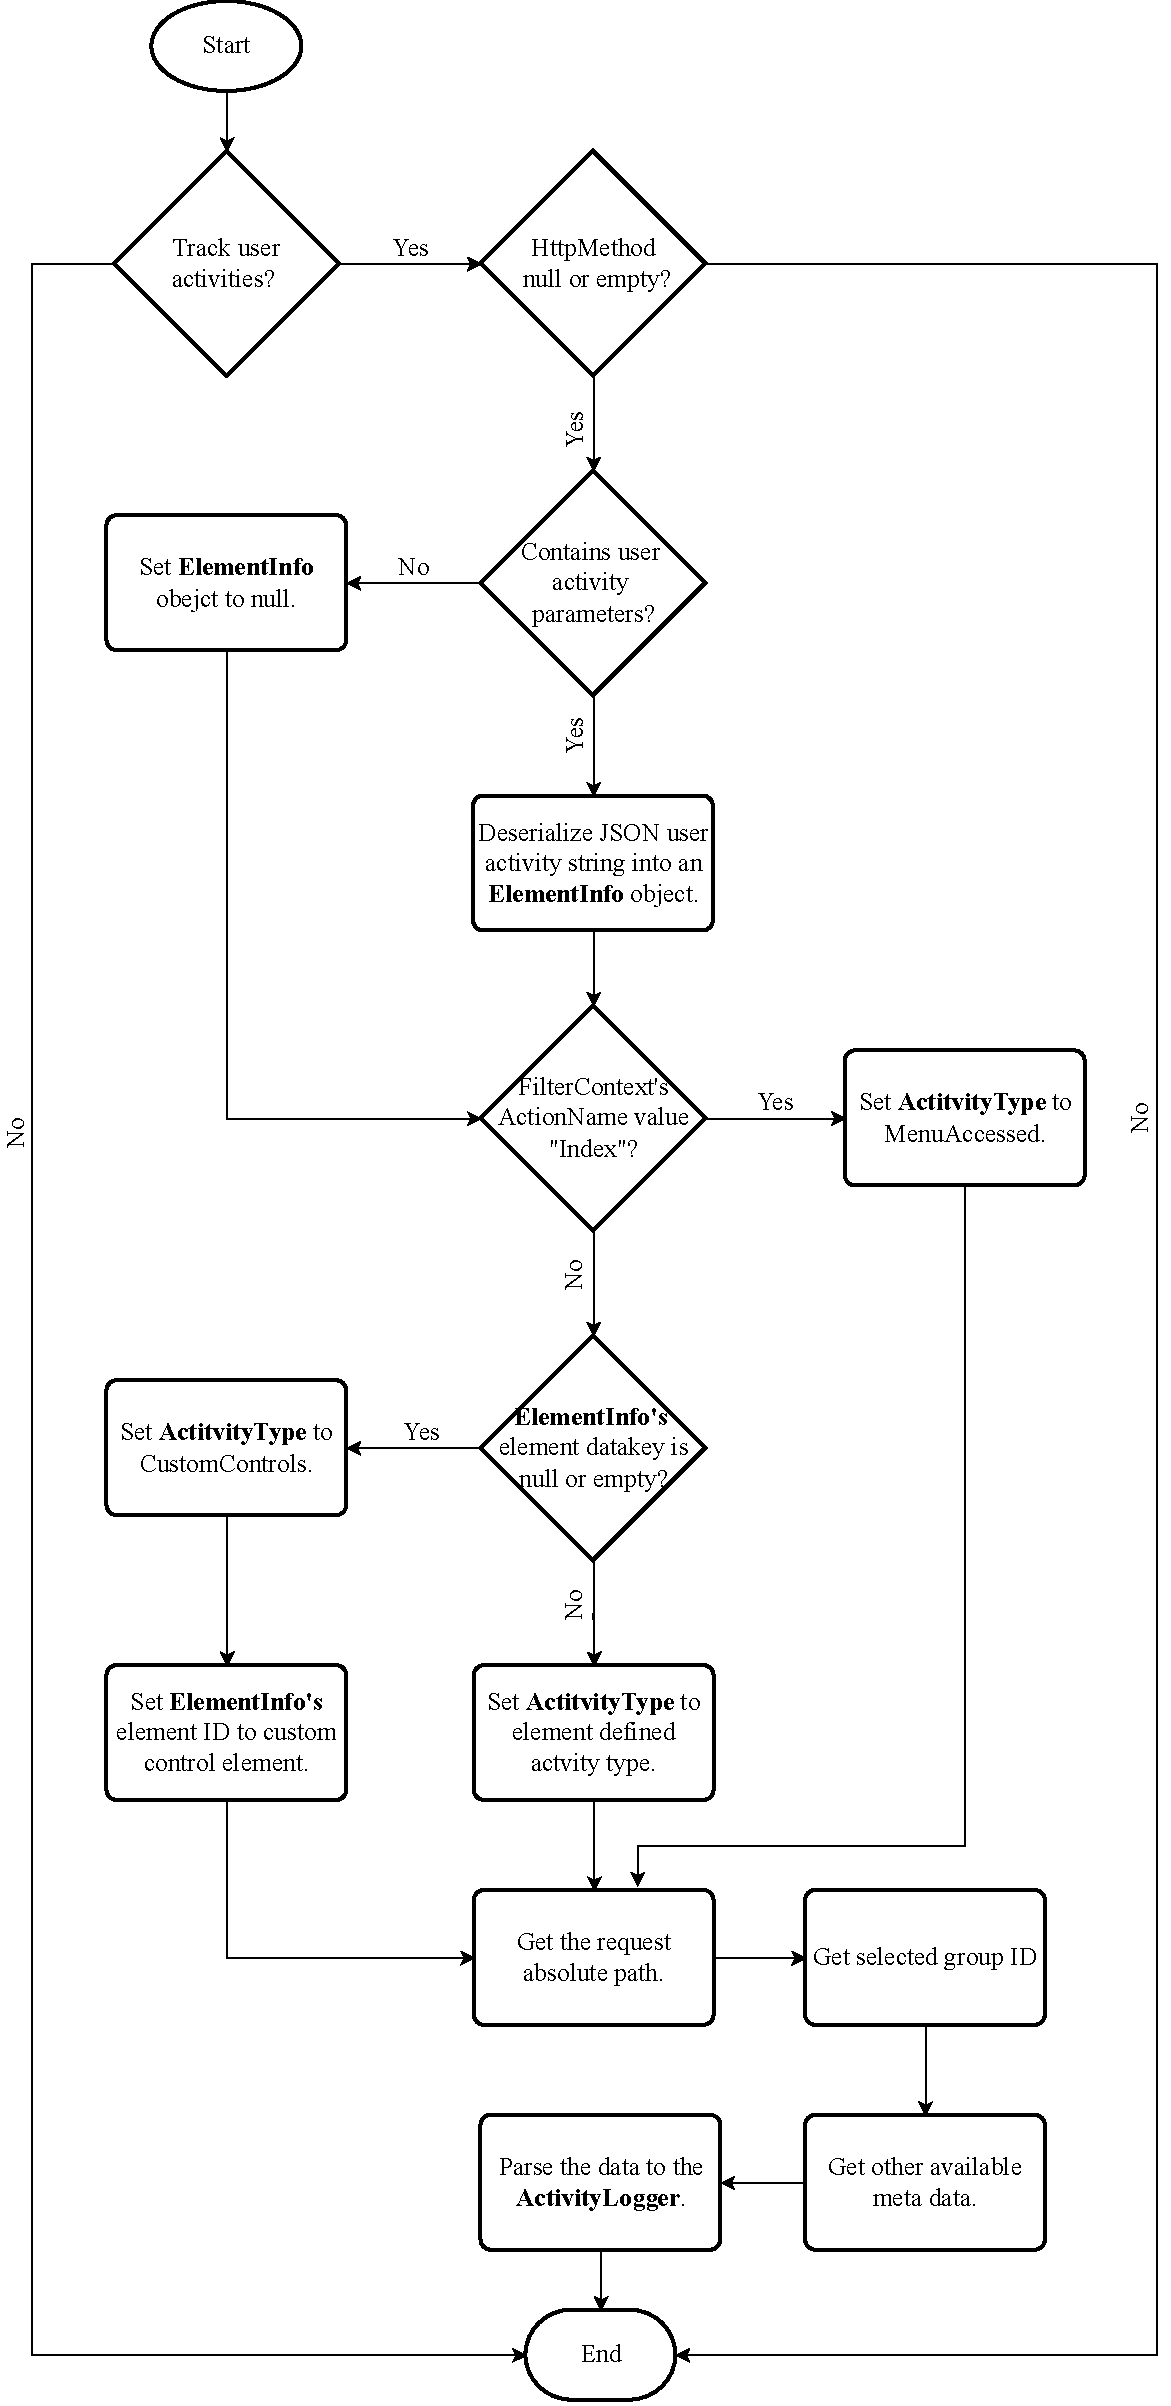
\includegraphics[width=0.95\textwidth]{Chapter2/SystemB_FilterContext/SystemB_FilterContext.pdf}
	\caption[Server-side log parsing flow diagram]
	{\textit{Server-side log parsing flow diagram}}\label{fig:ch2_loggingParse}
\end{figure}

\clearpage

If the \texttt{request header} contains the \texttt{Index} keyword, which is the first procedure that needs to be executed for a web page being accessed, the activity can be classified as accessing a system, subsystem, or web page. This activity type is the first user activity type at this point of the log parsing before it is processed again to another user activity type. \par If the request does not contain the \texttt{Index} keyword, the process will continue to the next operation that will check if the \texttt{ElementInfo}'s \texttt{ElementDataKey} is either a null or empty value. If there are any data available, the activity type can be set to the custom control defined activity type or custom control to represent the custom-made elements. The \texttt{ElementID} is set to the custom control element or the defined custom control's identification. \par If the \texttt{ElementInfo}'s \texttt{ElementDataKey} is null or an empty value, the user activity type is set to the element's defined activity type. After the activity type is resolved, the request origin of the user-based activity is obtained by getting the request's absolute path.\par After the request origin has been obtained, other relevant session information such as the group that represents a certain entity data can be obtained as well as the user's identification and other relevant metadata that is available at this stage to complete the log attributes that need to be captured from \Cref{tbl:ch2_keyLoggingAttributes} to complete the user-based activity log.\par The data are parsed to the activity logger that will write the log into a database if the log was successfully obtained. This will end the logging process until a new user-based event log is ready to be processed and stored in the database.

\clearpage

\subsection{Storage of event logs}
The log attributes in \Cref{tbl:ch2_SQLLoggingTable} will have foreign key references to other tables in the database for other tables, as seen in \Cref{fig:ch2_erdOfEventLogs}. 

\begin{figure}[!htb] % An h :here, t: top, b: bottom.
	\centering % cent the figure
	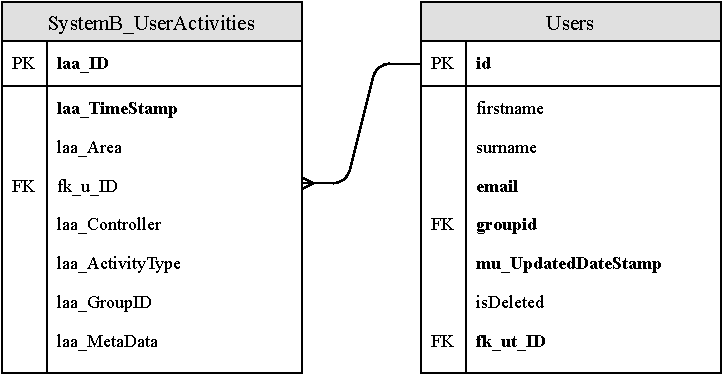
\includegraphics[width=0.8\textwidth]{Chapter2/SystemB_ERD_Basic/SystemB_ERD_Basic.pdf}
	\caption[ERD of user activities]
	{\textit{ERD of the user activities}}\label{fig:ch2_erdOfEventLogs}
\end{figure}

\Cref{fig:ch2_erdOfEventLogs} illustrates an ERD diagram that describes the relationship of the table created to store the log attributes with other relevant tables. This enables different fields of the other tables to be used to categorise the logs in the system utilisation analysis. \Cref{fig:ch2_database} illustrates the flow diagram of the database interaction to store the event log data.

\begin{figure}[!htb]
	\centering
	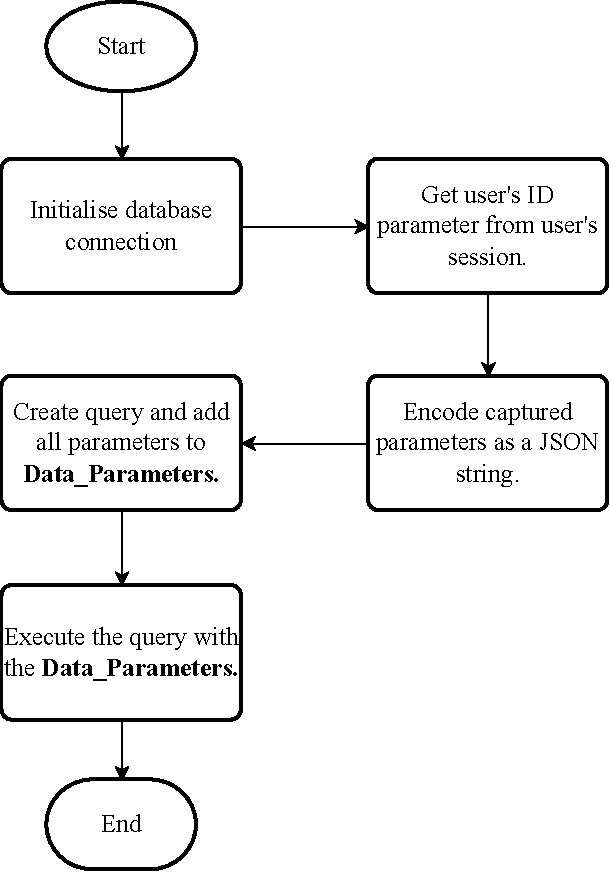
\includegraphics[width=0.43\textwidth]{img/Chapter2/sql_interaction/sql_interaction.pdf}
	\caption[Database interaction flow diagram]
	{\textit{Database interaction flow diagram}}\label{fig:ch2_database}
\end{figure}

\Cref{fig:ch2_database} illustrates how connection to the database is established. The user's identity is obtained from the active session, the obtained meta data are then converted into a JSON string for storing. The final query is built and executed to store in the relational database.

\subsection{Maintenance prioritisation}
The system utilisation analysis aims to provide maintenance recommendations to developers to improve their maintenance efforts by:

\begin{itemize}
	\item Prioritising maintenance efforts on systems that are more frequently used, and
	\item decommissioning new systems. User-based activities provide a quantitative reason why certain systems can be decommissioned due to inactivity of users.
\end{itemize}

This can be achieved by implementing maintenance prioritisation using \Cref{eq:ch2_maintenanceFactorSimplified} created from the functional requirements for maintenance prioritisation (\ref{fr:maintenanceFactor}):

\begin{equation}
	\label{eq:ch2_maintenanceFactorSimplified}
	M_{PF} = A_{N} \times P_{N}
\end{equation}

where:

\begin{itemize}
	\item $M_{PF}$ is the maintenance priority factor,
	\item $A_{N}$ is the normalised activity for the total logs obtained per subsystem, and
	\item $P_{N}$ is the normalised priority factor for the subsystem.
\end{itemize}

Normalised user activities per subsystem are described by \Cref{eq:ch2_eventNormalised}:

\begin{equation}
	\label{eq:ch2_eventNormalised}
	A_{N} = \frac{A_X - A_{Min}}{A_{Max} - A_{Min}},
\end{equation}

where:

\begin{itemize}
	\item $A_X$ is the total obtained user activities for the specified subsystem,
	\item $A_{Min}$ is the total minimum user activities for a subsystem, and
	\item $A_{Max}$ is a subsystem's total maximum user activities.
\end{itemize}

The normalised priority factor $P_N$ is described by \Cref{eq:ch2_priorityNormalised}:

\begin{equation}
	\label{eq:ch2_priorityNormalised}
	P_{N} = \frac{P_X - P_{Min}}{P_{Max} - P_{Min}},
\end{equation}

\begin{itemize}
	\item $P_X$ is the total obtained users that have access to the subsystem,
	\item $P_{Min}$ is the total minimum number of users that have access to any subsystem,
	\item $P_{Max}$ is the total maximum number of users that have access to any subsystem.
\end{itemize}

\clearpage

A normalised value for the priority is used because there is no predefined way to describe the importance of any subsystem. \Cref{fig:ch2_maintenancePriortisationFlow} illustrates the log-analysis flow diagram of implementing the maintenance prioritisation for a software system. 

\begin{figure}[!htb]
	\centering
	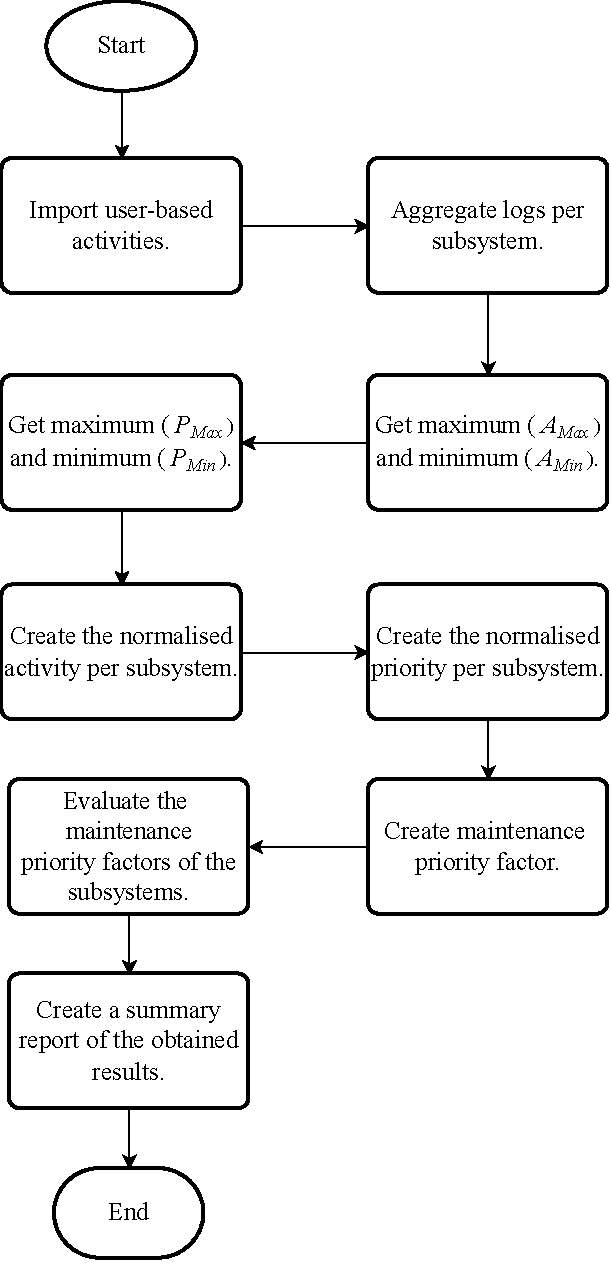
\includegraphics[width=0.68\textwidth]{img/Chapter2/maintenancePriortisation/maintenancePriortisation.pdf}
	\caption[Maintenance prioritisation flow diagram]
	{\textit{Maintenance prioritisation flow diagram}}\label{fig:ch2_maintenancePriortisationFlow}
\end{figure}

As can be seen in \Cref{fig:ch2_maintenancePriortisationFlow}, the user-based activity logs are imported into the log analysis tool from the relational database. The logs are aggregated into unique subsystems. The total number of user actions are counted as well as the total number of unique users associated with the captured logs. The maximum and minimum total user activities ($A_{Max}$ and $A_{Min}$) and users ($P_{Max}$ and $P_{Min}$) are obtained for the software system. \par The normalised activity ($A_N$) for each subsystem is created from the obtained activities. Normalised priority ($P_N$) is created from the maximum and minimum priority obtained. The maintenance priority factor is created from the normalised parameters for each system and is then evaluated. A summary report is created for the results obtained from the log analysis using the maintenance prioritisation method.

\clearpage

\section{Conclusion}
\Cref{sec:ch2_investigate} discussed the defined functional requirements for a logging mechanism for the system utilisation analysis outlined in \Cref{sec:ch2_logAnalysisTools,sec:ch2_utilisationImprovements}. The user activity types defined in \Cref{sec:ch2_userActivityTypes} are the basis for the log attributes that must be logged to create a user-based log. \par The log points capture the logs and send them to the server logging point where they are processed and stored in writing in a database.\par The logs are extracted into a visual presentation that enables maintenance improvement suggestions based on the use analysis in \Cref{sec:ch2_logAnalysisTools,sec:ch2_utilisationImprovements}.